% =====================================================================
%  Evolving Verifiers — NeurIPS 2027 Datasets & Benchmarks submission (anonymous)
%  v1.0 (673a): all numbers synced to the authoritative numbers artifact (schema 672h).
%  Engine: pdflatex/bibtex  (or tectonic).  Style: official neurips_2025.sty
% =====================================================================
\documentclass{article}

\usepackage[dandb]{neurips_2025}   % Datasets & Benchmarks track; anonymous by default
\usepackage[utf8]{inputenc}
\usepackage[T1]{fontenc}
\usepackage{hyperref}
\usepackage{url}
\usepackage{booktabs}
\usepackage{amsfonts}
\usepackage{amsmath}
\usepackage{amssymb}
\usepackage{graphicx}
\usepackage{xcolor}
\usepackage{tikz}
\usepackage{pgfplots}
\pgfplotsset{compat=1.17}
\usetikzlibrary{arrows.meta,positioning,shapes.geometric,fit,backgrounds}

% placeholder for results pending the baseline batch (kept visible on purpose)
\newcommand{\TODO}[1]{\textcolor{red}{\textbf{[TODO: #1]}}}
\newcommand{\cmark}{\textcolor{green!60!black}{\checkmark}}

\title{Evolving Verifiers: Failure-Driven Evidence\\ Acquisition with Auditable Provenance}

\author{%
  Anonymous Author(s) \\
  Affiliation \\
  Address \\
  \texttt{email} \\
}

\begin{document}
\maketitle

\begin{abstract}
When LLMs produce knowledge at near-zero cost, the bottleneck moves from \emph{generating correct
knowledge} to \emph{evolving verifiers}: a verifier is worn out by the very samples it has
graded. Existing self-evolving benchmarks evolve the \emph{items}; we evolve the \emph{verifier},
under an externally interruptible audit discipline. We present \textbf{Queyi}:
\emph{conclusion--evidence--recomputation} bound into a chain, with the verifier's own
\emph{failures} as the only legal input to evolution. Objects are \emph{executable C++
assertions}; verdicts are \emph{four-state}
(\texttt{pass}/\texttt{fail}/\texttt{unknown}/\texttt{contradict}); credibility comes from a
forced provenance/scope split and a kernel-independent reconciler. It has \textbf{67} verdict
rules and \textbf{42} real cards, \textbf{31} with evidence anchors (\textbf{Verifier Coverage
73.8\%}, 95\% CI [58.0, 86.1]), a \textbf{452}-event authority ledger, and Merkle roots over
\textbf{5} directories. \textbf{On the same samples}, blind holdout recall is \textbf{82.9\% (34/41, 95\% CI [67.9,
92.8])} and corpus measurable recall \textbf{62.5\% (40/64, [49.5, 74.3])} (layered read:
sanitizer 85.3\%, compiler-warn 50.0\%, cross-compile 16.7\%), versus a \emph{static caliber arm}
at \textbf{2.4\%}/\textbf{17.2\%} ($\Delta$ \textbf{+80.5pp} / \textbf{+45.3pp}) and an
instrument-level random proxy at \textbf{9.8\%}/\textbf{21.9\%} ($\Delta$ \textbf{+73.2pp} /
\textbf{+40.6pp}); exact McNemar $p\le3.0\times10^{-8}$, Cohen's $h\ge0.85$, $\Delta$ lower
bound $\ge$28.6pp. \textbf{Limitations:} the headline numbers depend on one WSL sanitizer
environment; samples remain few ($n{=}41/64$); newly added samples were merged \emph{after}
reveal; the static arm is a caliber re-binning and the random arm an instrument-level
proxy---so we claim \emph{auditability plus on-sample significance}, \emph{not} superiority over
real static detectors or a budget-matched random baseline.
\end{abstract}

% =====================================================================
\section{Introduction}
\label{sec:intro}
% =====================================================================
\paragraph{The problem: generation is easy, verification is not.}
When knowledge itself is generated in bulk by LMs, the bottleneck shifts from ``generating correct
knowledge'' to \emph{evolving verifiers that keep pace with generation}. A fixed yardstick is worn
out by memorization and contamination---and a verifier is domesticated by the very samples it has
graded. The real question is therefore not ``how do we verify this batch of knowledge,'' but
``how does a verifier evolve without grading its own homework, with every step of that evolution
independently auditable.'' We ground this paradigm claim in an executable setting. An LLM can emit
thousands of C++ technical assertions in minutes. They are \emph{numerous}
(manual review does not scale), \emph{plausible} (syntax, terminology and tone all look right),
and \emph{quietly wrong} (errors surface only under a specific compiler flag, compiler, or
platform). This creates an asymmetry---\textbf{generation cost tends to zero, verification cost
does not}---which is the starting point of this work. Executable evaluation of generated code has
precedent~\cite{chen2021humaneval}; our question differs---not whether code passes tests, but
whether a knowledge claim is true.

\paragraph{Motivation 1: high scores $\neq$ real ability.}
SWE-bench turned ``fix real GitHub issues'' into a standard yardstick~\cite{jimenez2024swebench},
but follow-up work is systematically negative: gains on SWE-bench-Verified are partly
\emph{memory rather than reasoning}---models locate files at up to 76\% within the repo but only
53\% outside it~\cite{liang2025illusion}; models score $3\times$ higher on SWE-bench-Verified
than on two sibling benchmarks~\cite{prathifkumar2025verified}; and SWE-MERA reports 32.67\% of
successful patches involving solution leakage and 31.08\% passing due to insufficient
tests~\cite{adamenko2025swemera}. \emph{Implication:} a verifier tested on its own data will
reproduce this failure, so we choose \textbf{external samples first}, \textbf{irreversible
blinding}, and \textbf{layered reporting}.

\paragraph{Motivation 2: AI-text detection answers the wrong question.}
DetectGPT~\cite{mitchell2023detectgpt} and watermarking~\cite{kirchenbauer2023watermark} answer
``was this text written by an AI?''---a signal that degrades with length/domain and is fragile to
paraphrase~\cite{sadasivan2023canai}. More fundamentally, \textbf{provenance and truth are
independent questions}: human-written C++ can be wrong, and AI-written derivations can be right.
\emph{Implication:} we do not detect provenance; we \textbf{test assertions} (compile, warn,
sanitize, cross-compiler diff, cross-optimization diff).

\paragraph{Motivation 3: provenance moved from good practice to obligation.}
EU Regulation 2024/1689 (AI Act), Article 50 imposes transparency obligations on generative AI
outputs~\cite{eu2024aiact}. This aligns with our design: \textbf{every piece of knowledge must
carry who generated it, who verified it, where the evidence is, and under what conditions it
holds}.

\paragraph{Contributions.}
(1)~\textbf{A formalization of failure-driven verifier evolution} (\S\ref{sec:method}): evolution
is an operator $E(\mathcal{C}_t, F_t)$ acting on the evidence-acquisition capability
$\mathcal{C}_t$ and driven \emph{only} by registered failures $F_t$, with three checkable
properties---\emph{monotonicity} (evolution never removes evidence capability), \emph{minimality}
(every new rule must trace to a registered failure), and \emph{auditability} (each step leaves the
chain \emph{failure} $\to$ \emph{rule} $\to$ \emph{re-test}).
(2)~\textbf{An information-structure analysis of the four-state verdict} (\S\ref{sec:method}):
verdicts partially encode the latent pair (claim truth $\times$ detector availability); merging
\texttt{unknown} into \texttt{miss} mixes unmeasurable samples into the denominator, merging it
into \texttt{pass} manufactures false confidence, and denominator $=$ catch $+$ miss is the only
caliber that does not contaminate the estimate.
(3)~\textbf{Three formal conditions for auditability} (\S\ref{sec:method}): \emph{origin
traceability} (every verdict decomposes into rule $\times$ evidence), \emph{state
reproducibility} (a third party can rebuild the verdict-time inputs from on-disk artifacts), and
\emph{tamper detectability} (any modification of a controlled directory moves the Merkle root).
A runnable instantiation (67 rules, a 452-event ledger, five controlled directories), the
evaluation protocol (\S\ref{sec:protocol}), and the open artifact with single-command
recomputation realize all three.

\paragraph{What we do \emph{not} claim.}
We do not claim a better C++ textbook, a stronger detector, or a formal proof. We do not claim
``the verifier got stronger'' unless that strengthening is measured on the \emph{same external
samples under the same caliber} (\S\ref{sec:exp}, Fig.~\ref{fig:evolution}).

% =====================================================================
\section{Related Work}
\label{sec:related}
% =====================================================================
We compress prior work into five lines (a seven-direction table is in Appendix~\ref{app:related}).
All comparisons are \emph{positional and qualitative}, not empirical claims about those systems.

\paragraph{(1) Self-evolving / contamination-resistant benchmarks (they evolve the \emph{items}).}
Benchmark Self-Evolving~\cite{wang2024benchmarkevolving}, ArenaBencher~\cite{liu2025arenabencher},
SWE-bench-Live~\cite{zhang2025swebenchlive}, DynaBench~\cite{kiela2021dynabench} and
LiveBench~\cite{white2024livebench} all fight ``the model memorized the items'', but they evolve
the \emph{object under test}; who judges, and whether the judgment is right, remains a fixed
test/oracle.

\paragraph{(2) Mutation-guided LLM test generation (the closest engineering form).}
ACH~\cite{foster2025ach} and MUTGEN~\cite{wang2025mutgen} turn mutation testing from an
\emph{evaluation} device into a \emph{generation} device; Cleverest~\cite{liu2025cleverest} does
just-in-time regression test generation. We \emph{reuse} the mutation-feedback idea as an internal
self-justification layer, but we \emph{refuse} to treat mutation score as a defect-detection rate.

\paragraph{(3) Self-verification / LLM-as-a-judge / formal verification (partly adopted, partly rejected).}
LLM-as-a-judge~\cite{zheng2023judging} is practical and scalable, but we use LLMs only to
\emph{propose candidates} and keep the \emph{judgment} fully programmatic. seL4~\cite{klein2009sel4}
and CompCert~\cite{leroy2009compcert} show that proof power can be extreme, at high human cost and
narrow coverage; we do not pursue formal proofs, only \emph{evidence that a third party can
recompute line by line}. The mutation-testing survey~\cite{jia2011mutation} informs our framework,
but only for the self-justification layer.

\paragraph{(4) Measurement governance, reproducibility, provenance (our methodological sources).}
Goodhart/Strathern~\cite{goodhart1975problems,strathern1997improving}, reward
hacking~\cite{skalse2022rewardhacking}, reward over-optimization~\cite{gao2023scaling};
Datasheets~\cite{gebru2021datasheets} and Model Cards~\cite{mitchell2019modelcards};
reproducibility reporting~\cite{pineau2021improving}; statistical methods~\cite{clopper1934use,
fisher1935design,mcnemar1947note,benjamini1995controlling,holm1979simple,cohen1960coefficient};
Merkle trees~\cite{merkle1988digital} and provenance auditing~\cite{kao2025constantsize,wang2026whoaudits}.

\paragraph{(5) Trained fact-checking models (the nearest neighbor where the \emph{judge} itself evolves).}
MiniCheck~\cite{tang2024minicheck} trains an efficient fact-checking model to judge whether LLM
output is supported by a grounding document---the representative case of \emph{the judge being
improved}: the evolved object is model weights, the strategy is distillation, and auditability
boils down to trusting the model's behavior. This is complementary to, not competing with, our
goal: MiniCheck evolves ``judging faster''; we evolve ``judging in a process a third party can
audit.'' Table~\ref{tab:positioning} (Appendix~\ref{app:tables}) positions six works along five
dimensions; the one-line version is that all prior lines evolve the \emph{items}, the \emph{tests},
the \emph{proofs} or the \emph{judge}, whereas we evolve the verifier's \emph{evidence-acquisition
capability} and require each step to be externally measurable.


\paragraph{What we are not.} Not benchmark evolution (we evolve the stick, not the items); not
mutation testing (mutation is only an internal self-justification component); not
self-verification (judgment is fully programmatic; meta-state is checked by an independent
reconciler); not RAG/text-similarity (we verify \emph{executable assertions}, not textual
resemblance).

% =====================================================================
\section{Problem Definition and Threat Model}
\label{sec:threat}
% =====================================================================
\paragraph{Formalization.}
A \emph{knowledge assertion} $a$ is a decidable statement plus a \emph{boundary triple}
$\langle D, P, F\rangle$ (input domain, preconditions, failure conditions). \emph{Evidence} $e$ is
a replayable observation (compiler version $+$ command $+$ optimization level $+$ output $+$
content-addressed hash). A \emph{verdict} is $v\in\{\texttt{pass},\texttt{fail},\texttt{unknown},
\texttt{contradict}\}$; \emph{verification capability} $\mathcal{C}$ is the set of available
evidence-acquisition means. Our goal is \textbf{not} to maximize $\Pr[v{=}\texttt{pass}]$ but to
maximize agreement with ground truth \emph{without ever disguising \texttt{unknown} as \texttt{pass}}.

\paragraph{Why four states.} ``Detector unavailable'' and ``detector says fine'' are different
knowledge states; formally the four states are the two orthogonal orders of Belnap's four-valued
logic~\cite{belnap1977useful} (\texttt{contradict} $\equiv$ \emph{Both}, \texttt{unknown}
$\equiv$ \emph{None}). Recording \texttt{unknown} as \texttt{miss} understates capability and pollutes
the denominator; as \texttt{pass} it creates a \emph{false pass} (the most dangerous); recording
\texttt{miss} as \texttt{unknown} hides a capability gap. Hence the \textbf{denominator is
$\text{catch}+\text{miss}$ (measurable samples)}; \texttt{unknown} is reported separately and
excluded; \texttt{not\_error} is a separate class. The caliber is stored in the artifact, not in
prose.

\paragraph{Sixteen threats (T1--T16).}
Table~\ref{tab:threats} (Appendix~\ref{app:tables}) lists all sixteen with mitigations and
residuals; \S\ref{sec:validity} quantifies them under the standard validity
layers~\cite{shadish2002experimental}. The four that bear most on our claims are \textbf{T8}
(budget selection bias), \textbf{T13} (peeking), \textbf{T15} (untrusted LLM channel) and
\textbf{T16} (small-sample poisoning); their residuals are precisely what the A0--A5 ablations
(\S\ref{sec:exp}) and the e-process protocol (\S\ref{sec:method}) are designed to bound.


\paragraph{Three focus threats.}
\textbf{(a) Construct: ``execution passed'' $\neq$ ``knowledge is correct.''} A \texttt{catch}
means only that a specific signal appeared under a specific fixture, flag and compiler---not that
the assertion is true or false. Empirically, the same ASan samples are optimized away under
\texttt{-O1} (no observable side effect) and reported immediately under \texttt{-O0}; switching the
pipeline from single- to dual-flag (\texttt{-O0}+\texttt{-O2}) moved recall \textbf{66.7\% $\to$
87.5\% with the detector unchanged}---\emph{the caliber changed, not the capability}.
\textbf{(b) Meta-Goodhart: the verifier optimizes its own metric.} When the \emph{measure of
verification capability} is produced by the verification system, the system can raise its score by
changing the caliber, changing the denominator, or turning red lights green, with no external
reference. A real incident: a batch changed the detector flag but \emph{did not rerun the
generator}; the artifact stayed on the old caliber while the paper reported \textbf{81.2\%
(13/16)}---a number that \emph{never appeared in any artifact}---and the then-\texttt{--check} did
not compare those fields, so it stayed green. \textbf{(c) Evaluation contamination.} Three forms:
sample leakage (T3); \emph{shared-criterion} labeling, where ground-truth labels and the criterion
are generated by the same rule, making the score an \emph{upper bound} (our counterfactual
operator's $F_1{=}1.0$); and unblinded expansion.

% =====================================================================
\section{Method}
\label{sec:method}
% =====================================================================
\begin{figure}[t]
\centering
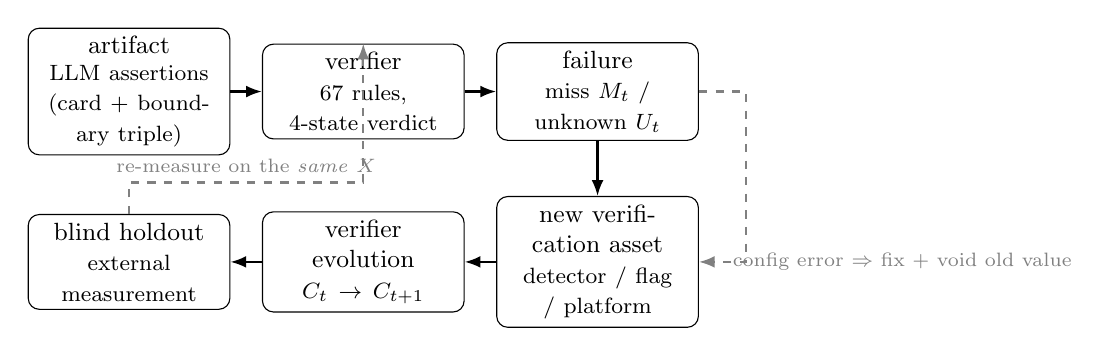
\begin{tikzpicture}[
  font=\small,
  box/.style={draw, rounded corners, align=center, inner sep=3pt, minimum height=9mm, text width=2.35cm},
  arr/.style={-{Latex[length=2mm]}, thick},
  fb/.style={-{Latex[length=2mm]}, dashed, thick, gray}
]
\node[box] (a) {artifact\\\footnotesize LLM assertions\\\footnotesize (card + boundary triple)};
\node[box, right=4mm of a] (b) {verifier\\\footnotesize 67 rules, 4-state verdict};
\node[box, right=4mm of b] (c) {failure\\\footnotesize miss $M_t$ / unknown $U_t$};
\node[box, below=7mm of c] (d) {new verification asset\\\footnotesize detector / flag / platform};
\node[box, left=4mm of d] (e) {verifier evolution\\\footnotesize $C_t \to C_{t+1}$};
\node[box, left=4mm of e] (f) {blind holdout\\\footnotesize external measurement};
\draw[arr] (a)--(b);
\draw[arr] (b)--(c);
\draw[arr] (c)--(d);
\draw[arr] (d)--(e);
\draw[arr] (e)--(f);
\draw[fb] (f.north) -- ++(0,4mm) -| node[pos=0.25, above, font=\scriptsize]{re-measure on the \emph{same} $X$} (b.north);
\draw[fb] (c.east) -- ++(6mm,0) |- node[pos=0.75, right, font=\scriptsize, align=left]{config error $\Rightarrow$ fix + void old value} (d.east);
\end{tikzpicture}
\caption{The failure-driven verification loop. Solid arrows form the main cycle; dashed arrows
are re-measurement and caliber correction. Tools: the rule engine (67 rules, four states), the
kernel-independent meta-state reconciler, and the counterfactual operator.}
\label{fig:loop}
\end{figure}

\paragraph{Architecture.}
\texttt{artifact}$\to$\texttt{verifier}$\to$\texttt{verdict}$\to$\texttt{ledger} (Fig.~\ref{fig:loop}).
\emph{Artifact}: knowledge cards, each with a boundary triple; a card lacking the triple may not
be pre-assigned a verdict (it should be \texttt{unknown}---a \emph{correct} output).
\emph{Verifier}: \textbf{67} rules produce four-state verdicts (two sources agree: engine rules
$=$ rule manifest). \emph{Evidence}: each compile/run stores content-addressed evidence (version
$+$ command $+$ flag $+$ output $+$ sha256); currently \textbf{28} cards have L1 evidence,
\textbf{28} are double-compiler confirmed, over \textbf{147} real compilations. \emph{Ledger}: a
\textbf{452}-event append-only authority ledger under a zero-change red line.

\paragraph{Four-state verdict.}
\begin{table}[t]
\caption{Four-state verdict.}
\label{tab:verdict}
\centering
\footnotesize
\begin{tabular}{@{}lll@{}}
\toprule
State & Meaning & Action \\
\midrule
\texttt{pass} & evidence supports the assertion; boundary triple complete & may enter the teaching ledger \\
\texttt{fail} & evidence contradicts the assertion & counterexample to the teaching set \\
\texttt{unknown} & insufficient evidence or detector unavailable & never recorded as pass/miss; reported separately \\
\texttt{contradict} & two pieces of evidence conflict (e.g.\ cross-compiler) & escalated to human review; no machine pick \\
\bottomrule
\end{tabular}
\end{table}
The point of \texttt{contradict} is that \emph{the machine never picks a side when evidence
conflicts}---the conflict itself is information. Machine cards are always
\texttt{needs\_review}$=$true and never counted as ``verified''; \texttt{verified} is
human-signed only.

\paragraph{Gate tiers L0/L1.} \textbf{L0 (blocking)}---meta-state reconciliation, gate-tier
legality, real-defect detection, blind-holdout state, unit tests---has \textbf{7} gates, all
passing stage-by-stage. \textbf{L1 (advisory)}---mutation score, boundary provenance,
supply-chain integrity---has \textbf{10} gates; red is registered, not blocking. Tiering
separates ``must hold'' from ``up for discussion''; putting everything at L0 invites relaxing
assertions to go green.

\paragraph{Provenance vs.\ semantic scope (forced split).}
\label{sec:prov}
\emph{Provenance} answers \emph{where an assertion comes from / who generated it} (generator
version, mutation-set hash, evidence sha256, compiler version). \emph{Semantic scope} answers
\emph{where it holds} (standard clause / compiler / platform / optimization level). They must be
split because a provenance-complete assertion can still be misused outside its scope (T6); writing
them together invites ``clear origin $\Rightarrow$ holds everywhere''. Current state (audit):
\textbf{26} boundary cards, provenance complete \textbf{26/26}, \textbf{semantic scope complete
0/26}---the mechanism is in place but scope backfill is essentially empty, which directly limits
external validity.

\paragraph{Meta-state reconciler (anti-self-justification).}
\label{sec:reconciler}
The reconciler is \emph{kernel-independent}: it rescans ground-truth sources (card fields,
directories, the rule engine) against the baseline, emitting \texttt{META-STATE-CONFLICT} and
exiting 1 on mismatch. Its discipline: assertions may hard-code a \emph{caliber}, never a
\emph{measurement}---via ground-truth alignment, additivity/partition
(\texttt{block}$+$\texttt{warn}$+$\texttt{advice}$=$total), or structural invariants. Residual:
``kernel-independent'' means it does not import the kernel, \emph{not} that a third party wrote it.

\paragraph{Failure-driven loop.} For every \texttt{miss}$\cup$\texttt{unknown} we attribute the
cause---a \emph{measurement-configuration error} (fix the config and \emph{void the old value}, not
a capability gain) or a \emph{capability gap} (add an evidence-acquisition means $\Rightarrow
C_{t+1}$)---then \textbf{re-measure on the same $X$} and quantify $\Delta$ with a CI; if $\Delta$
is not significant the addition does \emph{not} enter the claim table. Re-measuring on the same $X$
is essential, else ``capability gain'' is indistinguishable from ``an easier sample set''; a
budget-matched random control is essential because the gain may simply reflect \emph{more budget}.

\paragraph{Formal definitions (backing the three contributions).}
\emph{Verifier state} $\mathcal{C}_t$: the set of available evidence-acquisition means (detectors
$\times$ compilers $\times$ flags $\times$ platforms) at time $t$; its discrete form is the
67-rule set. \emph{Failure set} $F_t = \{x : v_t(x) \in \{\texttt{miss}, \texttt{unknown}\}\}$;
\texttt{miss} points directly at a capability gap, while \texttt{unknown} must first be attributed
(measurement-configuration error vs.\ capability gap). \emph{Evolution operator}
$\mathcal{C}_{t+1} = E(\mathcal{C}_t, F_t)$ with three checkable properties:
\emph{monotonicity} ($\mathrm{cov}(\mathcal{C}_{t+1}) \supseteq \mathrm{cov}(\mathcal{C}_t)$---
evolution never removes capability), \emph{minimality} (every application of $E$ must be triggered
by a \emph{registered} failure; no rule inflation without failure evidence), and
\emph{auditability} (each application leaves the triple (registered failure $f$, new rule $r$,
re-test record)). \emph{Information structure of the four states}: each sample carries the latent pair $(y, d)$
(claim truth $\times$ detector availability); \texttt{unknown} explicitly encodes
$d{=}\text{unavailable}$ and \texttt{contradict} inter-evidence conflict---hence merging
\texttt{unknown} into \texttt{miss} pollutes the denominator, merging into \texttt{pass}
manufactures false confidence, and denominator $=$ catch $+$ miss is the only non-contaminating
caliber. \emph{Auditability conditions}: origin traceability ($\forall v\, \exists (e,r): v = R_r(e)$),
state reproducibility (a third party rebuilds verdict-time inputs from on-disk artifacts), and
tamper detectability (any change to a controlled directory moves the Merkle root; the ledger is
append-only)---jointly necessary.

\paragraph{Rule-version pinning and e-process sequential testing.} We pin the ruleset by hashing
its canonicalised manifest (\texttt{rules\_manifest\_sha256}); the manifest exists today but the 452
ledger events do not yet carry the field (backfilling is future work). Because the ledger accumulates
item by item, we adopt an \emph{e-process} whose cumulative e-values multiply per item and stay
anytime-valid, so expansion needs no re-calibration (measured $2.5\times10^8$ / $2.5\times10^6$ for
the static / random contrasts, far above the threshold of 20). Details in Appendix~\ref{app:pinning};
neither is claimed as first---CELEUS~\cite{zhou2026celeus} already uses e-processes for a different
object and goal.\footnote{Anytime-validity costs a threshold of $\approx$20 versus $\approx$3.14, so
the e-value is a safety belt and cross-batch combiner, not our primary test.}

\paragraph{Two new metrics: Verifier Coverage and Evolution Efficiency.}
\textbf{Verifier Coverage (VC)} $=$ (real cards with evidence anchors) / (real cards). Real cards
are \texttt{atoms/**/ATOM-*.md} excluding \texttt{draft650/} (\textbf{42}, authority
\texttt{counts\_659.py}); ``evidence anchor'' means card status $\in$ \{verified,
red-team-verified, machine-verified\}, measured \textbf{31} ($23+3+5$; 11 drafts excluded).
$\Rightarrow$ \textbf{VC $=$ 31/42 $=$ 73.8\%} (Clopper--Pearson 95\% CI [58.0, 86.1]).
Per-domain: conc 3/3, hist 1/1, mem 22/24, ub 5/6, \textbf{lang 0/8} $\Rightarrow$ domain VC
$=$ 4/5---the language domain's 8 all-draft cards are the largest coverage gap (future work).
VC measures \emph{how much of the yardstick is genuinely graduated}: what fraction of the judged
semantic behaviors rest on evidence; it guards against ``rule-count inflation with hollow
evidence'' (complementing minimality).
\textbf{Evolution Efficiency (EE)} $=$ $\Delta$detection rate / $\Delta$rule count. Over the
auditable interval 660$\to$669 (blind recall 80.0\%$\to$87.5\%, rules 63$\to$67):
\textbf{EE $=$ 7.5pp / 4 rules $=$ 1.9pp/rule}; the mutation-core variant over the same interval
(62.5\%$\to$96.5\%) gives \textbf{8.5pp/rule}. \textbf{Double-caliber warning:} the two rates come
from \emph{different sample sets and different flag calibers in different batches}; EE is a
\emph{descriptive rate}, not a paired effect size---all main effects are read from the same-batch
McNemar / Cohen's $h$ (\S\ref{sec:exp}). EE is a historical observation; A0--A5 are the
experiments.

% =====================================================================
\section{Evaluation Protocol}
\label{sec:protocol}
% =====================================================================
The protocol is \emph{frozen before seeing results}; later changes must be logged with their effect
on existing numbers. Statistical details are in Appendix~\ref{app:stats}.

\begin{figure}[t]
\centering
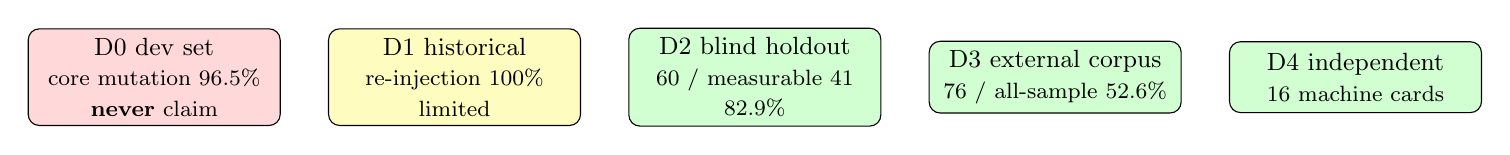
\begin{tikzpicture}[font=\small]
\node[draw, rounded corners, fill=red!15, align=center, minimum width=3.2cm, minimum height=9mm] (d0) {D0 dev set\\\footnotesize core mutation 96.5\%\\\footnotesize \textbf{never} claim};
\node[draw, rounded corners, fill=yellow!25, align=center, minimum width=3.2cm, minimum height=9mm, right=6mm of d0] (d1) {D1 historical\\\footnotesize re-injection 100\%\\\footnotesize limited};
\node[draw, rounded corners, fill=green!18, align=center, minimum width=3.2cm, minimum height=9mm, right=6mm of d1] (d2) {D2 blind holdout\\\footnotesize 60 / measurable 41\\\footnotesize 82.9\%};
\node[draw, rounded corners, fill=green!18, align=center, minimum width=3.2cm, minimum height=9mm, right=6mm of d2] (d3) {D3 external corpus\\\footnotesize 76 / all-sample 52.6\%};
\node[draw, rounded corners, fill=green!18, align=center, minimum width=3.2cm, minimum height=9mm, right=6mm of d3] (d4) {D4 independent\\\footnotesize 16 machine cards};
\end{tikzpicture}
\caption{Dataset layers D0--D4. Colour encodes whether external validity may be claimed
(red: never; yellow: limited; green: yes). D0 is self-justification only; D2 contains 10 unblinded
samples and D3 contains 20 (both merged after reveal, denominator only); D3 is further split into
layers A/B/C which must \emph{not} be merged.}
\label{fig:data}
\end{figure}

\paragraph{Dataset layers (D0--D4).}
Fig.~\ref{fig:data} summarises the five layers and their claim status; their current values are:
D0 core mutation \textbf{96.5\%} (self-justification only, never claimed), D1 re-injection 1/1
(coverage 12/15), D2 blind holdout \textbf{82.9\%} (34/41), D3 external corpus \textbf{62.5\%}
measurable (40/64; 52.6\% all-sample), and D4 16 machine cards (unsigned). The A/B/C sub-layers of
D3 must \emph{not} be merged into one number.

\paragraph{Baselines (three, all budget-matched).}
\label{sec:baseline}
\begin{table}[t]
\caption{Baselines and their alignment conditions.}
\label{tab:baseline}
\centering
\footnotesize
\begin{tabular}{@{}lp{5.2cm}p{6.4cm}@{}}
\toprule
Baseline & Definition & Alignment \\
\midrule
B1 static gate & static rules only (no runtime evidence) & same corpus, same verdict granularity \\
B2 static $+$ mutation & static rules $+$ mutation testing & same as above $+$ same mutation budget \\
\textbf{B3 budget-matched random} & random evidence acquisition under \emph{equal budget} & same budget (time/calls), same corpus, same flags \\
\bottomrule
\end{tabular}
\end{table}
B3 is the key control: it separates ``failure-driven'' from ``it just spends more''.
\textbf{Current status:} all three arms (static caliber re-binning, random$\dagger$ instrument-level
proxy, failure-driven) \emph{have been run on the same samples} (\S\ref{sec:exp}, $n{=}41/64$).
The \emph{true} B3 was wired through the split-repo \texttt{select\_assets} and run at 672g on the
older $n{=}21/48$; after the 672h expansion the random arm is again an instrument-level proxy, so we
claim \emph{direction}, not a controlled magnitude.

\paragraph{Ablation (A0--A5, restructured from the earlier A--F).}
The six groups, their pre-registered hypotheses, primary metrics and (placeholder) results are given
in Table~\ref{tab:e4} (\S\ref{sec:exp}); each group writes its hypothesis \emph{before} results.
Each group writes its hypothesis before results; a result contradicting the hypothesis is reported
as-is. \textbf{Current status: design frozen, 0 groups run} (this batch wrote scripts and design
only). \textbf{A0 - A5 is the key contrast.}

\paragraph{Metrics (seven).} Real-defect recall; blind-holdout recall; external recall; FPR;
mutation score (\emph{self-justification only}); regression-retention rate; cost. \textbf{Every
rate must carry a \texttt{denominator}}. Two \emph{descriptive} metrics of the verifier's own
state---Verifier Coverage and Evolution Efficiency (\S\ref{sec:method})---carry no detection-set
semantics and must not be read as detection rates.

% =====================================================================
\section{Experiments}
\label{sec:exp}
% =====================================================================
All numbers are \emph{recomputed from artifacts}; intervals are \textbf{Clopper--Pearson 95\%},
Wilson shown as sensitivity. Baseline arms are recomputed by a single script (see Appendix~\ref{app:repro}).

\begin{figure}[t]
\centering
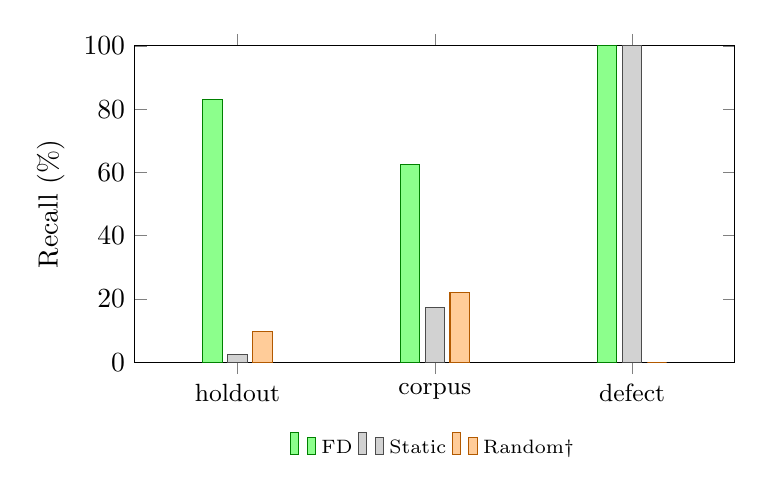
\begin{tikzpicture}
\begin{axis}[
  width=9.2cm, height=5.6cm,
  ybar, bar width=7pt,
  ymin=0, ymax=100,
  ylabel={Recall (\%)},
  symbolic x coords={holdout, corpus, defect},
  xtick=data,
  x tick label style={font=\small},
  legend style={font=\scriptsize, at={(0.5,-0.20)}, anchor=north, legend columns=3, draw=none},
  enlarge x limits=0.26,
  title style={font=\small},
]
\addplot[fill=green!45, draw=green!50!black] coordinates {(holdout,82.9) (corpus,62.5) (defect,100)};
\addplot[fill=gray!35, draw=gray!60!black] coordinates {(holdout,2.4) (corpus,17.2) (defect,100)};
\addplot[fill=orange!40, draw=orange!70!black] coordinates {(holdout,9.8) (corpus,21.9) (defect,0)};
\legend{FD, Static, Random$\dagger$}
\end{axis}
\end{tikzpicture}
\caption{Core recall across three arms (post-671a expanded samples; the holdout drop and corpus
rise are the honest re-estimates). \textbf{FD} (failure-driven) holdout
82.9\% [67.9, 92.8] and corpus 62.5\% [49.5, 74.3]; \textbf{Static} (rule-only, a
\emph{caliber re-binning}, not a re-run) 2.4\% [0.1, 12.9] / 17.2\% [8.9, 28.7];
\textbf{Random$\dagger$} (an instrument-level \emph{proxy}, not the paper's B3) 9.8\% / 21.9\%.
Bars show point estimates; Clopper--Pearson 95\% CIs are in Table~\ref{tab:e1}. $n=41/64$ is
still small, so read \emph{direction} first, magnitude second.}
\label{fig:core}
\end{figure}

\paragraph{E1 --- Main experiment: static vs.\ random vs.\ failure-driven.}
\begin{table}[t]
\caption{E1. Three arms on the same samples. Static is a caliber re-binning; Random$\dagger$ is a
proxy (the real B3 needs the split-repo \texttt{select\_assets}).}
\label{tab:e1}
\centering
\footnotesize
\begin{tabular}{@{}lp{2.7cm}p{2.4cm}p{1.7cm}p{1.5cm}@{}}
\toprule
System & Blind holdout (CP 95\%) & Corpus meas.\ (CP 95\%) & Defect & Control FPR \\
\midrule
Static (caliber re-bin) & 2.4\% (1/41) [0.1, 12.9] & 17.2\% (11/64) [8.9, 28.7] & 100\% (6/6) & --- \\
Random$\dagger$ (proxy) & 9.8\% (4/41) [2.7, 23.1] & 21.9\% (14/64) [12.5, 34.0] & N/A & --- \\
\textbf{FD (failure-driven)} & \textbf{82.9\% (34/41) [67.9, 92.8]} & \textbf{62.5\% (40/64) [49.5, 74.3]} & 100\% (6/6) & 18.2\% (2/11) [2.3, 51.8] \\
$\Delta$(static$\to$FD) & \textbf{+80.5pp} [68.4, 92.6] & \textbf{+45.3pp} [33.1, 57.5] & 0 & --- \\
$\Delta$(random$\dagger\to$FD) & \textbf{+73.2pp} [59.6, 86.7] & \textbf{+40.6pp} [28.6, 52.7] & N/A & --- \\
\bottomrule
\end{tabular}
\end{table}
\textbf{Expanded-sample honesty:} the expansion moved holdout 81.0\%$\to$\textbf{82.9\%} (up;
new subset 17/20 vs historical 17/21) and corpus 54.2\%$\to$\textbf{62.5\%} (up; new subset
14/16 vs historical 54.2\%); both rises are split into \emph{composition change} vs
\emph{within-layer change} and are \textbf{not} read as capability gains. The H4 subset
consistency check passes for holdout (+4.0pp) but \textbf{fails for corpus (+33.3pp, outside the
pre-registered range)} and is registered as a composition shift. FPR stayed at \textbf{18.2\%} (one new false
positive, sample h35, is registered). We report these as measured---no ``correction.''
\textbf{Pre-registered rule:} if the difference CI crosses 0, the ``failure-driven'' mechanism
does \emph{not} hold and must be reported as-is. All four $\Delta$ CIs are strictly positive
(lowest bound 28.6pp).

\paragraph{E2 --- Caliber ablation.} Three arms share the \emph{same raw catch counts}
(holdout 17, corpus 26; recomputed after the 671a expansion) and differ only in the denominator:
\begin{table}[t]
\caption{E2. Caliber ablation (same raw counts, different denominator). The 669d table
(87.5/82.4/82.4 and 43.8/37.8/35.0) is \emph{retired}: its denominators are the pre-expansion
16/17/40.}
\label{tab:e2}
\centering
\footnotesize
\begin{tabular}{@{}lp{3.6cm}p{3.6cm}p{3.6cm}@{}}
\toprule
Arm & Caliber & holdout (CP 95\%) & external (CP 95\%) \\
\midrule
\textbf{A (main; drop unknown)} & denominator $=$ catch$+$miss & \textbf{82.9\% (34/41) [67.9, 92.8]} & \textbf{62.5\% (40/64) [49.5, 74.3]} \\
B (unknown $\to$ miss) & denominator incl.\ detector-unknown & 81.0\% (34/42) [65.9, 91.4] & 54.8\% (40/73) [42.7, 66.5] \\
C (unknown $+$ not\_error) & denominator $=$ all samples & 81.0\% (34/42) [65.9, 91.4] & 52.6\% (40/76) [40.8, 64.2] \\
\midrule
$\Delta$(A$-$C) & & $+1.9$pp & $\mathbf{+9.9}$pp \\
\bottomrule
\end{tabular}
\end{table}
The caliber effect on the external corpus (up to \textbf{9.9}pp) is not negligible, so reporting
a rate without its caliber lets readers pick anywhere in 52.6--62.5\%.

\begin{figure}[t]
\centering
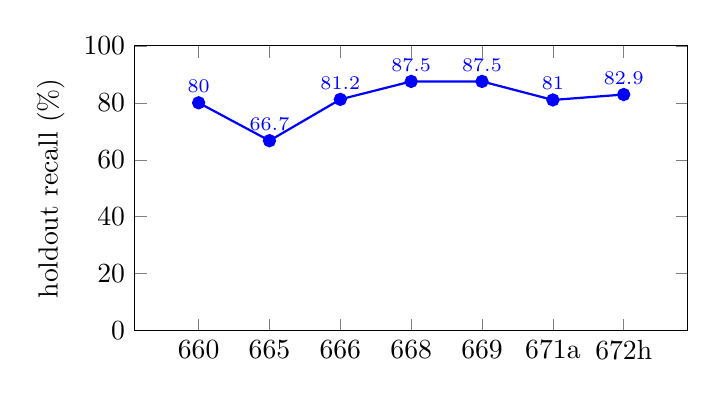
\begin{tikzpicture}
\begin{axis}[
  width=8.6cm, height=5.2cm,
  ymin=0, ymax=100, ylabel={holdout recall (\%)},
  symbolic x coords={660,665,666,668,669,671a,672h}, xtick=data,
  nodes near coords, nodes near coords style={font=\scriptsize},
  enlarge x limits=0.15,
]
\addplot[mark=*, thick, blue] coordinates {(660,80.0) (665,66.7) (666,81.2) (668,87.5) (669,87.5) (671a,81.0) (672h,82.9)};
\end{axis}
\end{tikzpicture}
\caption{Evolution curve. \textbf{80.0\% $\to$ 66.7\% $\to$ 87.5\% $\to$ 81.0\% is not a
capability curve}: 660 is a small denominator (20 samples / 7 true errors), 665 is single-flag
(30 samples / 17 true errors), 668 is dual-flag---with the detector unchanged; 671a is an
\emph{expanded-sample re-estimate} (16$\to$21 measurable, 10 unblinded samples merged in, corpus
caliber moved to dual-flag $+$ \texttt{setarch})---the 87.5$\to$81.0 drop is the measurement
object growing, not the verifier regressing. The 666 value (81.2\%) never landed in
any artifact and is marked hollow. 656/662 report only mutation metrics (core 62.5\% $\to$ 96.5\%).}
\label{fig:evolution}
\end{figure}

\paragraph{E3 --- Evolution curve.}
The holdout column is \emph{not the same $X$}, so it must not be read as evolution. The only
same-sample re-measurement is 668 vs.\ 665, and it changed the \emph{flag}, not the capability.

\paragraph{E4 --- Ablation framework (A0--A5; design frozen, experiments \emph{not} run).}
We re-express the pre-registered ablations as six \emph{same-batch-executable} groups A0--A5, each
with a written hypothesis (H) and a decision rule. Results are \emph{registered} as
\texttt{\{\{TODO\_ablation\_A0\}\}} \dots{} \texttt{\{\{TODO\_ablation\_A5\}\}}: this batch froze the
design and the scripts, it did \textbf{not} run the groups.
\textbf{The key contrast is A0 - A5} (failure-driven vs.\ same-budget random asset selection): it is
the paper's core-mechanism falsifier. \textbf{If the CI of $\Delta(\text{A0} - \text{A5})$ crosses
0, then ``failure-driven beats same-budget random'' does \emph{not} hold.} \textbf{A5's interface
was resolved at 672g} (split-repo \texttt{select\_assets}); the \emph{experiment} is not run. A1
needs a git-history ruleset snapshot; A2
hits the \emph{irreversible-blindness} barrier (once the holdout is revealed it cannot be re-blinded,
so a \emph{new} split is required). \textbf{Reality check:} at the current measurable $n=41/64$,
detecting $\Delta=15$pp needs $n\approx138$ (paired) / $\approx170$ per group (independent); the
$\pm10$pp half-width target needs $n=61/97$ and $\pm5$pp needs $n=236/378$. \textbf{Today the contrast still cannot yield an
interpretable $\Delta$.}

\paragraph{E5 --- Statistical tests for the baseline contrasts.}
FD and the two opponent arms are paired \emph{on the same samples} (holdout 21 pairs, corpus 48
pairs) $\Rightarrow$ exact McNemar; the effect size is Cohen's $h$~\cite{cohen1988statistical}
(recomputed after the 672h expansion):
Small-sample warning: McNemar significance rests on the extreme $c{=}0$ structure---a few reverse
pairs would inflate $p$ quickly; magnitudes remain interval-reads at $n=41/64$. The Cohen's-$h$
label discipline is in Appendix~\ref{app:stats}.

\paragraph{E7--E8 --- LLM judge arm and external anchor.}
An LLM judge arm (\textbf{GLM-4}) caught \textbf{12/12} errors vs.\ FD's 6/12 on the same subset
but produced \textbf{4/8 false positives} (\textbf{50\%}) on controls---\emph{more sensitive, far
less specific}; all four pre-registered hypotheses failed, which is the empirical case for T15 (an
LLM may \emph{propose}, but its output never becomes a verdict). An external anchor on the official
\textbf{C++ Core Guidelines} gives \textbf{44.0\%} over 50 snippets (verbatim 28.6\%, reconstructed
UB 80.0\%), with pre-registered \textbf{H2 missing by 0.8pp} and registered as \emph{not} passed.
Both experiments are detailed in Appendix~\ref{app:extra}; both are reported without
``correction''.\footnote{The LLM arm is a single model on a single prompt, and some samples carry
\texttt{answer\_leak\_risk}; the anchor's reconstructed subset is our own (\texttt{verified\_source=false})
and therefore an upper bound.}

% =====================================================================
\section{Analysis}
\label{sec:analysis}
% =====================================================================
\textbf{(1) Labels are the largest error source.} A batch reported ``20 holdout samples'' of which
only \textbf{7} were true errors: the same data reads 35\% or 80.0\% depending on the denominator.
The number jumped because the \emph{object being measured} was corrected, not because the verifier
improved. \textbf{(2) Environment dependence is the root cause of silent score drops.} Sanitizer
branches need a specific WSL environment; without it 15 samples degrade to \texttt{unknown} and
external recall falls \textbf{35.0\% $\to$ 10.0\%} while the guard stays green (it compares
artifact to front-end, not artifact to a real machine). \textbf{(3) ``Changed code without
rerunning'' is a systematic failure mode (three times):} a reported 81.2\% never landed; the
counterfactual $F_1$ was once 0 because the criterion was coded but the artifact not rerun; a
real-machine corpus rerun differed from the artifact by 10 catches.
\textbf{(4) Mutation score $\neq$ real defect detection.} Internal mutation core is \textbf{96.5\%}
(110/114; all-scope \textbf{81.8\%}, 130/159) while the external corpus is \textbf{62.5\%}
measurable (40/64; 52.6\% all-sample); Just et
al.~\cite{just2014mutants} show mutants are correlated with, but not equivalent to, real faults.
\textbf{(5) Whether failure-driven gains are real.} On the same samples FD beats the static
re-binning arm and the random-instrument proxy with exact McNemar $p\le3.0\times10^{-8}$ and Cohen's
$h\ge0.85$ (\S\ref{sec:exp}). The random arm is an \emph{instrument-level proxy} (the true B3 ran
only at 672g on the old $n{=}21/48$), so ``failure-driven beats same-budget random'' remains a
\emph{directional} conclusion---exactly what ablation A0--A5 is designed to test (\S\ref{sec:exp},
not run).

% =====================================================================
\section{Threats to Validity}
\label{sec:validity}
% =====================================================================

% =====================================================================
\section{Claim Boundary}
\label{sec:claim}
% =====================================================================

% =====================================================================
\section{Conclusion}
\label{sec:conclusion}
% =====================================================================
LLMs drive the \emph{generation} cost of technical knowledge to near zero, but the
\emph{verification} cost does not fall. We argue that verification cannot be solved by
model-judging-model (shared failure domain) or by AI-text detection (wrong question); it requires
binding \emph{verdict--evidence--recomputation} into a chain an external party can interrupt.
Queyi realizes this as four auditable mechanisms: four-state verdicts (\texttt{unknown} first
class), a forced provenance/semantic-scope split, a kernel-independent meta-state reconciler, and
a failure-driven verification loop.

We also made our own failures part of the method: 66.7\%$\to$87.5\% is a caliber change, not a
capability gain, and the old value must be voided; \textbf{81.0\%$\to$82.9\% and
54.2\%$\to$62.5\% are expanded-sample re-estimates, not capability gains}---both rose, and we
report them as measured, without ``correction''; 81.2\% never appeared in any artifact, and ``code
changed without rerun'' must be caught by the guard (and is \emph{not} caught today). A third-party
read-only audit rates overall credibility \textbf{6/10}: the infrastructure is trustworthy, the
\emph{numbers are fragile}.

\textbf{Evidence boundary.} The current evidence \emph{supports} ``verification capability can be
measured externally and failure-driven progress is traceable,'' and ``\emph{on the same samples}
FD significantly beats the static re-binning arm and the random-instrument proxy'' ($\Delta$
lower bound $\ge$28.6pp, exact McNemar $p\le3.0\times10^{-8}$, Cohen's $h\ge0.85$); it does
\emph{not} support ``better than a \emph{real} static detector or a true B3'' (split-repo
interfaces BLOCKED), ``generalizes to other languages'' (C++ only), ``exact magnitudes''
($n{=}41/64$ still small; $\pm$5pp half-width needs $n{=}236/378$), or \emph{any} ablation
conclusion (design frozen, experiments not run). \textbf{Future work:} (i) keep expanding toward $n\ge100$ (672h already moved holdout to 41
measurable / corpus to 64; ablation needs $n\approx103$--173 pairs); (ii) expose the split-repo
interfaces, run the true B1, and rerun the true B3 at the new denominator; (iii) run A0--A5 so that
A0$-$A5 can try to falsify the core mechanism; (iv) obtain at least one independent reproduction.

\label{page:endmain}% records the page where the main text ends (for the 9-page check)
\bibliographystyle{plainnat}
\bibliography{queyi_refs}

% =====================================================================
\newpage
\appendix

\section{LLM Arm and External Anchor (details)}
\label{app:extra}
\paragraph{E7 --- LLM judge arm (result \emph{opposite} to expectation, registered as such).}
A paired arm gave the same samples (6 catch $+$ 6 miss $+$ 8 control) to \textbf{GLM-4}
(temperature 0.01, prompt v1). It caught \textbf{12/12} errors vs.\ FD's 6/12 on the same subset, but
produced \textbf{4/8 false positives} (\textbf{50\%}) on controls (item-wise agreement 0.50; exact
McNemar favours the LLM, $b{=}0$, $c{=}6$, $p{=}0.031$). \textbf{All four pre-registered hypotheses
failed}: the LLM is \emph{more sensitive but far less specific}. Two caveats: some samples carry
\texttt{answer\_leak\_risk} (fixture comments may hint the answer), so ``judging'' cannot be fully
separated from ``reading the answer''; and it is a single model on a single prompt. This is the
empirical case for T15---an LLM may \emph{propose}, but its output never becomes a verdict.

\paragraph{E8 --- External anchor (C++ Core Guidelines; H2 misses by 0.8pp).}
We scanned the official \textbf{C++ Core Guidelines} (\texttt{isocpp/CppCoreGuidelines}, sha256
\texttt{27b53e7d\ldots}), taking one compilable snippet per rule in document order (87 rules). The two
subsets are reported \emph{separately} because their targets differ: \textbf{A} verbatim guideline
snippets (35 measurable, \textbf{28.6\%} [14.6, 46.3]) and \textbf{B} reconstructed UB fragments
(15, \textbf{80.0\%}); total \textbf{44.0\%} over 50. A is low because most guideline text is
stylistic advice rather than an executable error---``no detection'' there is \emph{expected}, not a
miss; B is our own reconstruction (\texttt{verified\_source=false}) and is therefore an \emph{upper
bound}. Pre-registered verdicts: H1/H3 hold, \textbf{H2 misses by 0.8pp} and is registered as
\emph{not} passed. A harness (\texttt{prelude\_v1}) was added post-registration because raw
compilability was 11/60; the deviation is logged and does not change hypotheses or thresholds.

\section{Threat, Validity and Evolution Tables}
\label{app:tables}
Layer read at 672h (k/n per layer; layers are never merged): corpus sanitizer
\textbf{85.3\%} (29/34), compiler-warn \textbf{50.0\%} (9/18), cross-compile \textbf{16.7\%}
(2/12)---three further layers lack local detectors and therefore claim \emph{no} rate; holdout
sanitizer \textbf{84.6\%} (33/39). These denominators are recomputed from the landed reveal
artifacts and are the source of the abstract's layered read.

\begin{table}[t]
\caption{E4. Ablation groups A0--A5. Each row writes its hypothesis \emph{before} results.}
\label{tab:e4}
\centering
\footnotesize
\begin{tabular}{@{}clp{3.3cm}p{3.6cm}l@{}}
\toprule
ID & Remove/change & Hypothesis & Primary metric & Result \\
\midrule
A0 & Full system (baseline) & --- & detection rate & \texttt{\{\{TODO\_ablation\_A0\}\}} \\
A1 & $-$failure-derived rules (post-657 ruleset) & H: detection drops & $\Delta$ detection vs.\ A0 & \texttt{\{\{TODO\_ablation\_A1\}\}} \\
A2 & $-$holdout isolation (blind$\to$dev) & H: overfitting (dev$\uparrow$, blind flat) & dev vs.\ blind recall & \texttt{\{\{TODO\_ablation\_A2\}\}} \\
A3 & $-$provenance (boundary-triple check) & H: false-pass rate rises & false-pass rate & \texttt{\{\{TODO\_ablation\_A3\}\}} \\
A4 & $-$mutation (L1 self-justification) & H: internal strength drops & mutation kill (internal) & \texttt{\{\{TODO\_ablation\_A4\}\}} \\
A5 & random-budget control & H: below A0 & $\Delta$ detection vs.\ A0 & \texttt{\{\{TODO\_ablation\_A5\}\}} \\
\bottomrule
\end{tabular}
\end{table}
\begin{table}[h]
\caption{E5. Paired contrasts on the same samples. $b$ = FD catch \& opponent miss;
$c$ = opponent catch \& FD miss. All four contrasts have $c=0$ (the opponent's catches are a
subset of FD's), so the difference comes entirely from samples only FD catches.}
\label{tab:e5}
\centering
\footnotesize
\begin{tabular}{@{}llrll@{}}
\toprule
Contrast & Set & $(b, c)$ & exact McNemar $p$ & Cohen's $h$ \\
\midrule
FD vs.\ Static & holdout ($n{=}41$) & (33, 0) & $2.3\times10^{-10}$ & \textbf{1.98} (large) \\
FD vs.\ Static & corpus ($n{=}64$) & (29, 0) & $3.7\times10^{-9}$ & \textbf{0.97} (large) \\
FD vs.\ Random$\dagger$ & holdout ($n{=}41$) & (30, 0) & $1.9\times10^{-9}$ & \textbf{1.65} (large) \\
FD vs.\ Random$\dagger$ & corpus ($n{=}48$) & (24, 0) & $1.2\times10^{-7}$ & \textbf{1.24} (large) \\
\bottomrule
\end{tabular}
\end{table}

\section{Rule Pinning and e-Process (details)}
\label{app:pinning}
\textbf{Rule-version pinning (design principle; manifest-level today).} Rules inevitably evolve, so
a ledger that records only verdicts cannot let a third party recompute a one-year-old decision: the
ruleset of the day must be pinned. We snapshot the ruleset and hash the canonicalised manifest into
\texttt{rules\_manifest\_sha256}, archived append-only, with each ledger event double-referencing
that hash and the evidence-toolchain snapshot. \textbf{Current state (measured):} the manifest
exists (\texttt{rules\_sha256}, version 1.0.0, 67 rules), but the \textbf{452 ledger events do not
yet carry the field}---backfilling is registered as future work, so today a historical recomputation
must \emph{assume} the ruleset was unchanged.

\textbf{e-process sequential testing (an implemented preliminary).} The ledger accumulates items one
at a time, yet rates are reported at snapshots---that is \emph{peeking}. We treat each event as a
binary observation, mix likelihood ratios over a grid of alternatives, and obtain an \emph{e-process}
(a non-negative supermartingale with expectation 1 under $H_0$); the cumulative e-value is
\emph{multiplied} by one factor per new item, and we reject when $\sup_t e_t \ge 1/\alpha$ (i.e.\ 20
at $\alpha{=}0.05$). Ville's inequality guarantees that peeking at \emph{any} time keeps the
type-I error at $\alpha$, so expansion needs no re-calibration, and the e-values \emph{multiply
across batches}---isomorphic to an append-only ledger. Measured, the FD contrasts reach e-values of
$2.5\times10^8$ / $1.8\times10^7$ (static) and $3.5\times10^7$ / $2.5\times10^6$ (random), far
above the threshold of 20. \textbf{Honest boundaries:} the anytime-valid price is a threshold of
$\approx$20 versus $\approx$3.14 for a single fixed-sample test ($\approx$6.4$\times$ in
likelihood-ratio terms), so the e-value here is a \emph{safety belt for expansion and a cross-batch
evidence combiner}, not the primary test; and the implementation is a preliminary not yet in CI.
\textbf{Difference from CELEUS}~\cite{zhou2026celeus}: CELEUS uses e-processes to \emph{save
samples} in LLM evaluation; we use them for anytime-valid, third-party-recomputable decisions over a
\emph{knowledge-assertion} ledger. We do \emph{not} claim to be first.


\begin{table}[t]
\caption{Positioning: six works $\times$ five dimensions. Benchmark evolution evolves the
\emph{items}; MiniCheck evolves the \emph{judge} (a trained fact-checking model); Queyi evolves
the \emph{verifier's evidence-acquisition capability} while requiring every step of that
evolution to be externally measurable.}
\label{tab:positioning}
\centering
\footnotesize
\begin{tabular}{@{}p{2.5cm}p{2.2cm}p{2.6cm}p{2.2cm}p{2.1cm}p{2.0cm}@{}}
\toprule
Work & Object evolved & Strategy & Auditable & Failure-driven & 4-state \\
\midrule
Benchmark Self-Evolving~\cite{wang2024benchmarkevolving} & items / samples & model-feedback rewriting & partial (generation logs) & no (pass/difficulty signal) & no \\
ArenaBencher~\cite{liu2025arenabencher} & items (adversarial) & opponent-model games & partial & no (win-rate signal) & no \\
LiveBench~\cite{white2024livebench} & items (periodic refresh) & human $+$ model updates & partial (item dates) & no (temporal rotation) & no \\
SWE-bench Verified~\cite{jimenez2024swebench,liang2025illusion} & items (human filtering) & manual subset curation & high (human review) & no (static set) & no \\
MiniCheck~\cite{tang2024minicheck} & the judge (fact-check weights) & distillation training & no (trusts the model) & no (training objective) & no \\
\textbf{Queyi (ours)} & \textbf{verifier capability $\mathcal{C}$} & \textbf{failure-driven: \texttt{miss}/\texttt{unknown} $\to$ new detectors/rules} & \textbf{Merkle $+$ 452-event ledger $+$ per-sample detail} & \textbf{yes (only legal input)} & \textbf{yes (\texttt{unknown}/\texttt{contradict} first-class)} \\
\bottomrule
\end{tabular}
\end{table}
\begin{table}[t]
\caption{What the current evidence does and does not support.}
\label{tab:claim}
\centering
\small
\begin{tabular}{@{}p{1.3cm}p{5.4cm}p{7.0cm}@{}}
\toprule
 & Claim & Evidence \\
\midrule
\cmark\ supported & High recall on \emph{seen} error types & holdout \textbf{82.9\%} (34/41) [67.9, 92.8]; corpus measurable \textbf{62.5\%} (40/64) [49.5, 74.3] (post-672h) \\
\cmark\ supported & Gates catch \emph{known} defects (change a number, go red) & range self-check 5/5 red; gate \texttt{overall=PASS} \\
\cmark\ supported & Provenance chain fully auditable & 5 Merkle roots consistent; 452-event ledger unchanged; provenance triple landed \\
\cmark\ supported & Caliber declarable and recomputable & three-arm caliber ablation; every rate carries a denominator \\
\cmark\ supported & On the same samples FD beats the static re-binning and random$\dagger$ proxy arms & exact McNemar $p\le3.0\times10^{-8}$; Cohen's $h\ge0.85$; $\Delta$ lower bound $\ge$28.6pp (\S\ref{sec:exp}) \\
\cmark\ supported & Verifier semantic coverage and evolution rate are measurable & Verifier Coverage 31/42 = 73.8\% [58.0, 86.1] (domain 4/5); EE 1.9pp/rule (descriptive; \S\ref{sec:method}) \\
\midrule
$\times$ not supported & Generalization to \emph{unseen} error types & all samples same-source; scope backfill 0/26 \\
$\times$ not supported & Absolute ``detection rate $X$\%'' & $n{=}41/64$, CI half-width $\approx$12pp; $\pm$5pp needs $n{=}236/378$ \\
$\times$ not supported & Better than a \emph{real} static detector / true B3 & static arm is a caliber re-binning; random$\dagger$ is a proxy; real interfaces BLOCKED; 0 ablations run \\
$\times$ not supported & ``$F_1{=}1.0$ is calibrated'' & criterion and truth are same-source $\Rightarrow$ upper bound \\
$\times$ not supported & Mutation score as detection rate & core 96.5\% $\neq$ defect-detection rate~\cite{just2014mutants} \\
$\times$ not supported & Evolution trend & only a single same-sample re-measurement \\
\midrule
\multicolumn{3}{@{}p{13.7cm}@{}}{\textbf{Not reproducible (fail when the environment changes):} holdout/external recall depend on \textbf{WSL + g++ + \texttt{setarch}} (silent drop 35.0\%$\to$10.0\% without WSL; 669d-era caliber); TSan results are intermittently unavailable under WSL high-entropy ASLR; the OTS anchor is a zero-attestation placeholder, so ``anchored on-chain'' does \emph{not} hold.} \\
\bottomrule
\end{tabular}
\end{table}

The three tables below are moved here to keep the main text within the 9-page limit; their labels are unchanged, so all cross-references still resolve.

\begin{table}[t]
\caption{Threats, mitigations and residual risks.}
\label{tab:threats}
\centering
\small
\begin{tabular}{@{}p{0.5cm}p{4.6cm}p{4.2cm}p{4.6cm}@{}}
\toprule
\# & Threat & Mitigation & Residual \\
\midrule
T1 & Self-justification (toolchain proves itself) & kernel-independent reconciler (\S\ref{sec:reconciler}) & reconciler still needs human review; \texttt{--check} $\neq$ independent implementation \\
T2 & Self-made distribution bias & blind holdout + external corpus (D2/D3) & small external sample \\
T3 & holdout leakage & irreversible reveal; holdout dir not scanned & 10 appended samples have no blinding \\
T4 & developer-knowledge bias & independent generation (A/B/C) & same-process context; not truly independent \\
T5 & caliber drift & meta-state reconciliation & covers registered fields only \\
T6 & semantic-scope misuse & forced provenance/scope split (\S\ref{sec:prov}) & scope completeness 0/26 \\
T7 & metric confusion (mutation $\to$ detection) & metric layering; mutation is self-justification only & external readers may still misread \\
T8 & selection bias (budget) & budget-matched random baseline (\S\ref{sec:baseline}); three arms \textbf{run} & random arm is an \emph{instrument-level proxy} (true B3 not rerun at 672h) \\
T9 & overfitting historical defects & blind D2 + external D3 & appended samples unblinded \\
T10 & reproducibility crisis & Merkle roots + version capture + time anchor & OTS is a placeholder; WSL dependency undeclared \\
T11 & authority manipulation & 452-event ledger, zero-change red line & discipline, not cryptographic enforcement \\
T12 & unclear AI authorship & AI-use registry & contribution split remains a convention \\
T13 & \textbf{peeking / selective stopping}: the ledger accumulates while rates are reported at snapshots & frozen statistical plan; \textbf{e-process / confidence sequence} as a pre-committed expansion protocol (\S\ref{sec:method}) & nothing forces $\mu_0$ to be fixed in advance $\Rightarrow$ pre-registration required \\
T14 & \textbf{four-layer contamination}: literal / near-duplicate / semantic / procedural---can be ``inflated but reproducible'' & paired counterfactual probes (rename identifiers, change compiler/order); unsealing event log; four-layer de-duplication & passive cleaning is unreliable; probes need human reading \\
T15 & \textbf{untrusted LLM channel}: prompt injection / adversarial input (CVE-2025-59145 CamoLeak, CVSS 9.6; indirect-injection ASR 24--52.77\%) & prompt-level spotlighting/datamarking; structural schema check; \textbf{architectural: LLM output never becomes a verdict, ML detection warns but never blocks} & touch-point registry not done; the LLM arm's false-positive rate is 50\% (\S\ref{sec:exp}) \\
T16 & \textbf{small-sample poisoning}: \textbf{250} malicious samples (0.00016\% of tokens) reliably plant a backdoor---the decisive variable is the \emph{absolute count}; our $n{=}41/64$ lies in that range & canary cards; paired counterfactual probes; the reconciler uses a \emph{different} dependency set; candidates run sandboxed as untrusted code & no safety margin; passive cleaning unreliable (3\% poisoning moves the error rate 3\%$\to$24\%) \\
\bottomrule
\end{tabular}
\end{table}
\begin{table}[t]
\caption{Five validity layers: threat / mitigation / residual.}
\label{tab:validity}
\centering
\small
\begin{tabular}{@{}p{1.8cm}p{4.4cm}p{4.0cm}p{3.6cm}@{}}
\toprule
Layer & Threat & Mitigation & Residual \\
\midrule
Construct & \texttt{catch} $\neq$ truth; A/B/C split by detector availability not difficulty; mutation score not a detection proxy~\cite{just2014mutants}; \textbf{static arm is a caliber re-binning, not a re-run; random$\dagger$ is an instrument-level proxy, not B3} & caliber/denominator/opt\_levels/env stored with artifacts; dual-flag; three-state separation; proxy arms marked $\dagger$ and excluded from conclusions & cross-environment reproduction unverified (upgraded from ``residual'' to ``observed failure'': score drops without WSL); no independent label review; ``with/without runtime evidence'' vs.\ ``failure-driven'' not yet separated (needs ablation) \\
Internal & meta-Goodhart; budget selection bias; code changed without rerun & caliber three-step discipline; range self-check (5/5 turn red); budget-matched random control & guard does not rerun the detector, so the 666 incident can recur; ablation design frozen, 0 groups run \\
External & small $n$ (holdout 21 / corpus 48 measurable); \textbf{expanded samples merged after reveal (no blind state: 10 holdout $+$ 20 corpus)}; same-source clustering; scope 0/26; single domain (C++) & layered reporting; two sample sets explicitly incomparable; unblinded samples explicitly flagged & static re-bin $+$ random$\dagger$ proxy \emph{run}; \textbf{real B3 BLOCKED}; 0 ablations; reconciler is still our own; 0 third-party reproductions \\
Statistical & \textbf{small $n$ (41/64)} $\Rightarrow$ still-wide CIs; McNemar rests on the extreme $c{=}0$ structure; \textbf{control FPR 18.2\% (2/11)}; multiple comparisons; Wald invalid at small $n$; clustering; $p$ without effect size & frozen plan; CP primary, Wilson sensitivity; Fisher/Boschloo $+$ exact McNemar \emph{tool-implemented}; BH/Holm; difference $+$ CI $+$ effect size $+$ e-value required & $\pm$5pp needs $n{=}236/378$; $\pm$10pp needs $61/97$; $\Delta{=}15$pp needs $n\approx103$--173 (paired); magnitude not readable as exact; IRR not done \\
Temporal & OTS anchor expired~\cite{opentimestamps}; sample aging; environment drift (TSan intermittently fails under WSL high-entropy ASLR) & Merkle roots $+$ hash chain; versions captured with evidence & OTS not really anchored; re-pinning invalidates the anchor; WSL hard dependency undeclared \\
\bottomrule
\end{tabular}
\end{table}
\begin{table}[t]
\caption{E3. Cross-batch key metrics.}
\label{tab:e3}
\centering
\small
\begin{tabular}{@{}llp{3.0cm}lp{3.0cm}@{}}
\toprule
Batch & New capability & holdout (true/caliber) & mutation core & Nature \\
\midrule
656 & core PBT/mutation & --- & \textbf{62.5\%} (30/48) & mutants out of range \\
660 & trace layer & true 7, \textbf{80.0\%} (small den.) & --- & label over-claim \\
665 & expand 20$\to$30 & true 17, \textbf{66.7\%} (single flag) & --- & denominator changed \\
666 & claimed dual & \textit{81.2\% never landed} & --- & code changed, no rerun \\
668 & dual-flag rerun & \textbf{87.5\%} (14/16) & --- & \textbf{caliber change} \\
669 & caliber ablation $+$ CI & 87.5\% [61.7, 98.4] & \textbf{96.5\%} (110/114) & mutation still internal \\
671a & expansion $+$ corpus dual-flag & \textbf{81.0\%} (17/21) [58.1, 94.6] (10 unblinded merged) & --- & \textbf{expanded re-estimate} \\
672h & re-expansion (21$\to$41 / 48$\to$64) & \textbf{82.9\%} (34/41) [67.9, 92.8] (20 unblinded merged) & --- & \textbf{expanded re-estimate (H4 corpus shift registered)} \\
\bottomrule
\end{tabular}
\end{table}

\section{Rule Manifest (67 rules)}
\label{app:rules}
The rule engine computes \texttt{len(RULES)}$=$\textbf{67}. By severity: \textbf{block 44 / warn 16
/ advice 7} (total 67). By kind: fact 61 / pedagogy 5 / meta 1. Fields:
\texttt{id, title, severity, kind, quadrant, scope, automated, basis, fix\_hint, check}.
\emph{Correction note:} an earlier draft wrote ``67 (block 0 / warn 176 / advice 55)''; recomputation
gives \textbf{44/16/7} (sum 67), and the old triple cannot be reproduced from the rule table. The
full 67-row list is generated by the command in Appendix~\ref{app:repro} and shipped with the
supplementary material.

\section{Statistical Caliber (frozen)}
\label{app:stats}
\begin{table}[h]
\caption{Frozen statistical caliber.}
\centering
\small
\begin{tabular}{@{}lp{9.5cm}@{}}
\toprule
Scenario & Method \\
\midrule
Single-proportion CI & \textbf{Clopper--Pearson exact 95\%} (primary); Wilson (sensitivity); small-$n$ Wald \textbf{forbidden} \\
Independent comparison & \textbf{Fisher exact / Boschloo} \\
Paired (before/after) & \textbf{exact McNemar} \\
Multiple comparisons & exploratory \textbf{BH-FDR}; confirmatory \textbf{Holm}; family pre-defined \\
Effect size & \textbf{difference $+$ CI} mandatory \\
Clustering & estimate ICC/DEFF/$n_{\text{eff}}$; same-source cards $\neq$ independent observations \\
IRR & Cohen's $\kappa$~\cite{cohen1960coefficient} / Krippendorff's $\alpha$~\cite{krippendorff1980content}; $\ge$0.67 for tentative conclusions \\
\bottomrule
\end{tabular}
\end{table}
Formulas: Clopper--Pearson via the Beta quantile,
$\text{CI}=[B(\alpha/2;\,k,\,n{-}k{+}1),\,B(1{-}\alpha/2;\,k{+}1,\,n{-}k)]$; exact McNemar via the
binomial tail on discordant pairs. Red lines: no ``significantly better''; do not write
``ineffective'' for $0/8$; do not call a mutation kill-rate a detection rate; do not call a
same-criterion $F_1{=}1.0$ ``calibrated''. All criteria are recomputed, never copied from
artifacts. Residual-risk-to-gate mapping: Construct$\to$boundary gate; Internal$\to$caliber-consistency
gate; Statistical$\to$frozen-stats gate; External$\to$baseline gate; Temporal$\to$time anchor (placeholder).

\paragraph{Effect-size labels (\textbf{medium}, not ``large''---and how the label moved).} Cohen's
$h$ thresholds are negligible $<$0.2 / small 0.2 / medium 0.5 / large $\ge$0.8. An earlier draft
labelled the then-headline corpus effect $h=0.72$ ``large''; by threshold it is \textbf{medium}.
After the 672h expansion the recomputed corpus effect is $h=\textbf{0.97}$, which \emph{does} fall
in the large band---but this time the number and the label moved \emph{together}, and the rule
stands: \textbf{labels must follow thresholds, not narrative} (reading 0.72-medium and 1.98-large
as one magnitude was exactly the error to avoid).

\paragraph{Sample size (recomputed, Cohen~\cite{cohen1988statistical}; paired via
Connor~\cite{connor1987sample}).}
\begin{table}[h]
\caption{Recomputed sample size (power $1-\beta=0.8$, two-sided $\alpha=0.05$).}
\label{tab:samplesize}
\centering
\small
\begin{tabular}{@{}lrr@{}}
\toprule
Design & Difference & $n$ (per group) \\
\midrule
Two independent proportions & 0.35$\to$0.50 & 170 \\
Two independent proportions & 0.35$\to$0.55 & 96 \\
Two independent proportions & 0.35$\to$0.45 & 376 \\
Paired (exact McNemar, $\psi{=}0.3$) & 0.35$\to$0.50 & 103 \\
Paired (exact McNemar, $\psi{=}0.4$) & 0.35$\to$0.50 & 138 \\
Paired (exact McNemar, $\psi{=}0.5$) & 0.35$\to$0.50 & 173 \\
\midrule
CI half-width target & $\pm10$pp & 61 (holdout) / 97 (corpus) \\
CI half-width target & $\pm5$pp & 236 (holdout) / 378 (corpus) \\
\bottomrule
\end{tabular}
\end{table}
At the current measurable $n=41/64$ (post-672h expansion) the $\pm5$pp half-width needs
$n=236/378$ (gaps: holdout 195, corpus 314); a $\Delta=15$pp paired contrast needs
$n\approx138$, an independent one $\approx170$ per group. These are why the key ablation contrast
A0 - A5 is reported as a design, not a result.

\section{Per-sample Detail}
\label{app:persample}
For each primary metric we ship an \texttt{id}$\to$\texttt{verdict} table (the key to third-party
recomputation): holdout (\texttt{planted/detector/verdict/opts\_seen}), external
(\texttt{verdict/layer}), counterfactual (\texttt{ground\_truth/operator\_prediction/agree}),
mutation (\texttt{killed/survived}). Each table carries \texttt{env} (WSL/g++/setarch),
\texttt{caliber} (\texttt{opt\_levels}) and \texttt{denominator}.

\section{Reproduction Commands}
\label{app:repro}
\begin{verbatim}
# environment self-check (last two decide whether holdout/external can be reproduced)
python --version; node --version; g++ --version; wsl --status
# headline numbers
python tools/holdout_reveal_3_665.py        # pre-expansion caliber 87.5%  (requires WSL; superseded by the line below)
python tools/external_corpus_reveal_665.py  # pre-expansion caliber 35.0%  (requires WSL; superseded by the line below)
python tools/mutation_test_656.py           # core 96.5% / all 81.8%
python tools/counterfactual_extend_665.py   # F1=1.0
python tools/run_658_gate.py                # L0 5/5
# post-672h authority numbers: holdout 82.9% (34/41), corpus measurable 62.5% (40/64), FPR 18.2% (2/11)
python -c "import json;d=json.load(open('data/experiments/reveal_update_671a.json',encoding='utf-8'));print(json.dumps(d['pending_for_671b'],ensure_ascii=False,indent=2))"
# Verifier Coverage: denominator 42, numerator 31 -> 73.8% [58.0, 86.1]
python tools/counts_659.py --json           # atoms_real = 42 (denominator authority)
python -c "import sys;sys.path.insert(0,'tools');from stat_bounds import cp_interval;print(cp_interval(31,42))"
# consistency
python -c "import sys;sys.path.insert(0,'tools');import gate_engine;print(len(gate_engine.RULES))"  # 67
wc -l data/authority/decision_event_v2_ledger.jsonl  # 452
\end{verbatim}
Paths are relative to the artifact root (the non-anonymous release provides the full layout).
\texttt{reveal}-type commands must redirect their output to a temporary directory outside the repo.

\section{AI Use Statement}
\label{app:ai}
This draft was \emph{assisted} by an LLM; the human authors own the topic, structure, claim
boundaries and final decisions. A per-item registry is shipped with the artifact. In the first
batch the LLM performed structural compression, data-fill validation, citation verification,
anonymization and terminology unification; in the second batch (number update $+$ novelty
enhancement) it updated all numbers from \texttt{reveal\_update\_671a.json}
(\texttt{pending\_for\_671b}), added the two computed metrics (VC/EE), and rewrote the title,
abstract, intro positioning, contributions and related-work table---\emph{no} unlanded numbers
were introduced, no expanded-sample result was ``corrected'', and no ``first-ever'' claims were
made. Any unregistered AI contribution is treated as an undeclared author.

\section{Related Work (seven directions)}
\label{app:related}
\begin{table}[h]
\caption{Seven related-work directions.}
\centering
\small
\begin{tabular}{@{}lp{10.5cm}@{}}
\toprule
Direction & Representative work \\
\midrule
1 self-evolving / anti-contamination & Benchmark Self-Evolving~\cite{wang2024benchmarkevolving}; ArenaBencher~\cite{liu2025arenabencher}; SWE-bench-Live~\cite{zhang2025swebenchlive}; DynaBench~\cite{kiela2021dynabench}; LiveBench~\cite{white2024livebench} \\
2 mutation-guided LLM testing & ACH~\cite{foster2025ach}; MUTGEN~\cite{wang2025mutgen}; Cleverest~\cite{liu2025cleverest} \\
3 self-verification / LLM-judge & LLM-as-a-judge~\cite{zheng2023judging} \\
4 measurement governance / reproducibility & Datasheets~\cite{gebru2021datasheets}; Model Cards~\cite{mitchell2019modelcards}; reproducibility report~\cite{pineau2021improving}; Goodhart~\cite{goodhart1975problems,strathern1997improving} \\
5 formal verification $+$ LLM & seL4~\cite{klein2009sel4}; CompCert~\cite{leroy2009compcert}; LLVM+Lean~\cite{liao2026llvmlean}; Can LLMs Enable Verification~\cite{shefer2025canllms}; Formal Disco~\cite{poesia2026formaldisco} \\
6 LLM code error taxonomy & All Smoke No Alarm~\cite{banik2026allsmoke}; Uncovering Weaknesses~\cite{lian2024uncovering}; Pair Programming~\cite{lyu2025pairprogramming} \\
7 provenance \& auditability & Merkle~\cite{merkle1988digital}; Constant-Size Crypto Evidence~\cite{kao2025constantsize}; Who Audits the Auditor~\cite{wang2026whoaudits}; NeurIPS Dataset Review~\cite{wu2024neurips} \\
\bottomrule
\end{tabular}
\end{table}

\end{document}
